\chapter{SDN中LDoS防御方案设计}
\label{cha:design}
本章的主要内容为LDoS防御方案的设计。首先,对LDoS的特征进行分析,找到防御LDoS的关键点。然后,根据防御LDoS的要点,结合SDN的优势设计了SDN中防御LDoS的两种方案。最后,对两种方案的设计思想和实现方案进行探索和分析。本文是基于SDN中最经典的OpenFlow协议完成设计的。

\section{SDN中LDoS防御的关键点分析}
\label{chap4:keyanalysis}
前文已经对LDoS攻击的攻击形式进行了说明,本文首先分析单攻击源的LDoS攻击实现的关键点并找到合适的防御机制。LDoS攻击的核心思想就是通过周期性的引发TCP流丢包,触发TCP拥塞控制机制或者超时重传机制降低TCP流的吞吐量,最后达到以极低的流量使TCP流异常的目标。因此,本文防御LDoS有两种核心思想,第一种是采取措施使TCP流不丢包,第二种是找到并限制攻击源。

第一种思想是采取措施使得TCP流不丢包。通过前文可知,TCP流的丢包是由于LDoS的速率太高拥塞队列导致的。所以,只要交换机保护TCP流的最低通信需求,则TCP不会因为收不到任何包而进入超时重传状态。在SDN网络中,带宽保障可以通过SDN中特有的meter规则去实现,使用meter规则限制其他流的最高速率从而给TCP流提供有最低速率保障,则LDoS无法通过拥塞队列强迫TCP流完全丢包。从而达到防御LDoS攻击的效果。但是,这样的做法在LDoS攻击的突发到达的时候,速率依然会降得很低,而拥塞窗口也会相应的减小,因此,这种思想只能减轻攻击所造成的危害,但是不能完全消除LDoS攻击对TCP流的影响。

第二种思想是找到并且限制攻击源。在SDN网络中,所有的数据转发都是由流表规则匹配完成的,因此,在SDN中可以实现流级别的数据分析。由于LDoS攻击拥塞了某个交换机的队列才能实现攻击,因此,可以在交换机的端口处检测LDoS是否存在。LDoS攻击作为一个周期性的“方波”是能够由周期性来确认的,因此,在端口处只要能够确认有周期性的吞吐量变化,就能够确认攻击,再之后通过流级别的分析判断攻击流,最后,再对判断出来的攻击流的攻击源进行限制。使用这种思想来防御LDoS攻击就能够完全消除LDoS攻击流对TCP流的影响,但是,在攻击开始的时候TCP流会受到一定的影响,可能会出现部分TCP流进入超时重传状态,影响吞吐量。

\section{SDN中基于带宽保障的LDoS防御方案}
\label{chap4:bandguatee}

为了保证TCP流不进入超时重传状态,防御方案必须保证TCP流无论在什么情况下都不能丢包,结合SDN的特性,该方案结合OpenFlow的Meter规则来实现,可以最大程度利用SDN网络可以自由制定网络规则的特性。

首先,分析Meter规则是如何在SDN中运行的,才能制定相应的Meter规则防御LDoS攻击。Meter规则允许SDN实现各种各样的服务质量(Quality of Service,QoS)配置,其中就包括了速率限制。Meter规则能够直接与SDN中的流表规则绑定,这样Meter规则可以测量和控制所有与之绑定的流表规则的聚合速率,因此,Meter规则可以用来限制除TCP流以外的所有流聚合的速率。

\begin{table}[htbp]
	\centering  % 显示位置为中间
	\caption{Meter规则}  % 表格标题
	\label{table:meter}  % 用于索引表格的标签
	%字母的个数对应列数,|代表分割线
	% l代表左对齐,c代表居中,r代表右对齐
	\begin{tabular}{|c|c|c|}  
		\hline  % 表格的横线
        Meter Identifier & Meter Bands& Counters \\  % 表格中的内容,用&分开,\\表示下一行
        \hline
		
	\end{tabular}
\end{table}
%英文斜体字?
表\ref{table:meter}为SDN的Meter规则的主要内容。Meter Identifier是一个32比特的无符号整数,它能够用于唯一标识一个Meter规则。counters是统计与meter绑定的流表规则的统计相关数据,随时更新。其中,最重要的是Meter Bands,它是Meter规则控制和限制绑定聚合流的速率和处理包方式的部分。需要注意的是,每个Meter规则可以匹配多个Meter Band。表\ref{table:meterbands}为一个Meter Band部分,它由五个部分组成,首先是Band Type部分,这直接定义了速率超过限定速率以后,后面的包是如何处理的。此处有两种选项:一种为drop,这样它该Meter规则就可以被用来限制速率;另一种为dscp remark,这样就能增加数据包IP头中DSCP字段的丢弃优先级,可用于定义不同级别的服务。第二个参数是Meter规则限制的速率,它定义Meter规则最低适用的速率,若是速率高于该参数的数据包则需要根据Meter规则进行处理。Counters表示被该Meter Band处理的包的统计数据。Burst参数是本文需要调的一个重要参数,该参数定义了Meter Band的粒度。Type specific arguments表示band types有特殊的参数。


\begin{table}[htbp]
	\centering  % 显示位置为中间
	\caption{Meter Band}  % 表格标题
	\label{table:meterbands}  % 用于索引表格的标签
	%字母的个数对应列数,|代表分割线
	% l代表左对齐,c代表居中,r代表右对齐
	\begin{tabular}{|c|c|c|c|c|}  
		\hline  % 表格的横线
        Band Type & Rate & Burst & Counters & Type specific arguments \\  % 表格中的内容,用&分开,\\表示下一行
        \hline
		
	\end{tabular}
\end{table}

此方案使用Meter规则来实现对非TCP流的速率限制,这样就能够对LDoS攻击进行限制。但是,由于LDoS攻击具有一定的特殊性,普通配置Meter规则无法限制LDoS攻击,需要特殊的配置。首先,由于LDoS攻击会拥塞某个端口的队列,所以,对于每个激活的端口,都应当配置一个相应的Meter规则进行限制,对于从端口处发送非TCP数据的流表规则需要与该端口的Meter规则进行绑定,受该Meter规则的束缚。接下来,Meter规则的粒度也需要特殊的配置,默认的状态下,Meter规则是以1秒作为统计单位进行速率限制的,由于LDoS攻击的平均速率并不能满足Meter规则限制的需求,因此Meter Band设置的Burst参数需要重新配置。接下来,需要设置Rate参数的大小来限制非TCP聚合流的速率,设置的参数数值大了会影响其他正常流的速率,设置的值过小会使TCP流的窗口降至极小的程度,达不到限制LDoS攻击的效果。因此,研究该参数对吞吐量大小的影响非常重要。


基于带宽保障的LDoS防御方案可以分为两个模块完成。流程图如\ref{fig:meter-solution}所示。防御方案的第一模块为预配置Meter规则模块,控制器首先会检测所有激活端口,并给每个端口分配一个Meter规则,Meter规则需要调节Burst参数使得粒度在RTT级别大小,这样才能够有效的限制LDoS攻击的速率。其次,设置合理的Rate参数保证TCP流不进入超时重传机制的同时使滑动窗口不至于变得太小。设置Band Type为drop,这样就可以丢弃所有超速的包,保障了TCP流有一定的带宽可以使用。防御方案的第二个模块为流处理模块,有一个流进入交换机,则需要对该流进行区分处理。若是该流为TCP流,则该TCP流的流表不需要绑定任何Meter规则,这样它就不会被Meter规则所束缚,可以按照TCP拥塞控制的机制进行速率的控制。若是该流不是TCP流,则需要绑定Meter规则以保证该流不会对TCP流造成损害,特别是当该流为LDoS攻击流的时候,由于速率被控制,队列不会被该流所拥塞而造成TCP流丢包,TCP流就不会进入超时重传状态。


%图 窗口与burst size的关系图,窗口与限制速率关系	有无防御机制吞吐量对比图

\begin{figure}
    \centering
    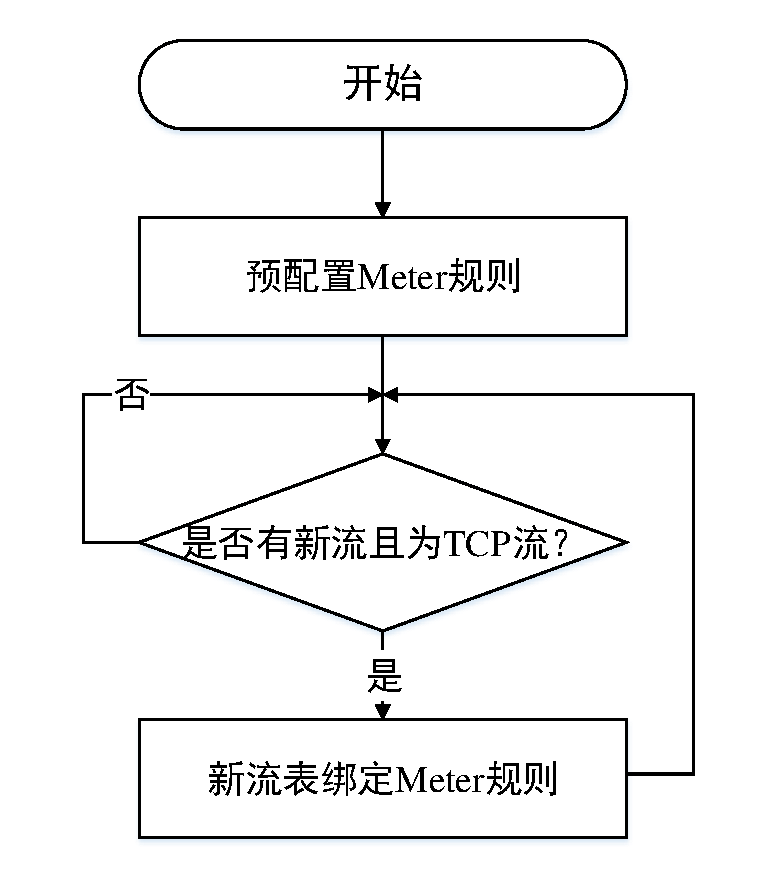
\includegraphics[scale=0.5]{meter-solution}
    \caption{基于带宽保障的LDoS防御方案流程图}
    \label{fig:meter-solution}
\end{figure}


\section{SDN中基于动态周期性检测的LDoS防御方案}
\label{chap4:SoftGuard}
已有SDN防御方案无法对LDoS限制的时候,为了保证SDN网络的正常传输,本文提出了基于动态周期性检测的方案。作为一个基于SDN的轻量级防御方案,该方案能够准确地识别并且有效地限制LDoS攻击。该方案分为三个模块,异常检测模块、攻击定位模块和攻击限制模块。每个模块都有特定的攻击,只有在一定的条件下激活才能发挥作用。因此,也最大程度的减轻了系统的负担。该方案是基于SDN中流表规则实现的,通过流表规则,SDN控制器能够获取交换机中各种有用的信息。

\subsection{SDN中相关流表规则分析}
\label{chap4:flowruleanalysis}

流表规则是SDN交换机中很重要的部分,所有的经过交换机的数据包都需要经过流表规则进行处理,这些数据包会优先寻找优先级比较高的流表规则进行匹配,这些流表规则可能有很多指令规则,其中比较重要的有两种,一种是将包从端口转发出交换机,另一种是转给交换机内的其他流表规则处理。表\ref{table:flowrule}为流表规则的主要内容。根据需求合理的配置流表规则的参数,能够实现对LDoS攻击的检测与限制。

本文对流表规则中重要的部分进行分析,制定合适的特制流表来防御LDoS攻击。在流表规则中,最重要的三个部分是匹配域(Match Fields)、优先级(Priority)和指令(Instructions)。匹配域一般是由入端口和数据包头部组成,也有其他可选项区域。优先级(Priority)是用来区分数据包优先匹配的规则的,若是同一个数据包同时匹配两个流表规则的匹配域,则该数据包会优先按照优先级高的流表规则的指令操作。通过匹配域和优先级可以使数据包确定匹配的流表规则,若是没有匹配上流表规则,就会将该数据包的包头上传控制器,请求相应的流表规则。在确认了流表规则之后,该数据包会按照流表规则的指令完成操作。流表规则还具备数据统计的功能,其中的计数器(Counters)就记录了很多重要的信息,其中包括了转发的数据包的数量和字节数,每当匹配到数据包时,计数器中的数据就会实时更新。流表规则中的Timeouts参数包括两个timeout参数,idle\_timeout和hard\_timeout。idle\_timeout若是一个非0的数值,则流表规则将在匹配最后一个包之后的idle\_timeout给定的时间后移除;idle\_timeout为0,则该参数不影响流表规则。hard\_timeout若是为非0的数值,则流表规则不管有没有匹配数据包,都会在hard\_timeout给定的时间后移除;hard\_timeout为0,则该参数不影响流表规则。若是idle\_timeout和hard\_timeout都为0,则流表规则永远存在,而且除了特定的指令外不会被删除。Cookie部分是控制器用于标识流表的不透明数据,该数据可以用来获取特定流表规则的信息,在处理数据包的时候不适用。Flags字段可用于出发特殊的消息给控制器。


\begin{table}[htbp]
	\centering  % 显示位置为中间13
	\caption{流表规则}  % 表格标题
	\label{table:flowrule}  % 用于索引表格的标签
	%字母的个数对应列数,|代表分割线
	% l代表左对齐,c代表居中,r代表右对齐
	\begin{tabular}{|c|c|c|c|c|c|c|}  
		\hline  % 表格的横线
        Match Fields & Priority & Counters & Instructions & Timeouts & Cookie & Flags \\  % 表格中的内容,用&分开,\\表示下一行
        \hline
		
	\end{tabular}
\end{table}

控制器通过以恒定的速率进行周期性的查询,可以获得每个流表规则中计数器的速率。对于不同应用,通过选择合适采样的周期可以尽可能减少控制器的带宽负载,同时也可以尽可能提高服务的质量。本文将每次查询的间隔时间长度标记为$T_s$,将以此采样间隔内的平均速率当做采样时刻的速率,用于不同的服务。公式\ref{eqa:rate}展示了从流表规则的数据中获取流表规则速率的方式。

\begin{equation}
	\label{eqa:rate}
	S(t) = \frac{Counter\_bytes(t) - Counter\_bytes(t - T_s)}{T_s}
\end{equation}

\subsection{总体设计}
\label{chap4:overview}

基于动态周期性检测的LDoS防御方案有三个模块,异常检测模块、攻击定位模块和攻击限制模块。整体框架如图\ref{fig:architecture}所示。其中异常检测模块是在交换机中给每个端口都安装了特制的流表规则用于统计检测TCP的聚合流量。由于异常检测模块并没有对所有流表规则进行检测,这样就减少了对于控制器的带宽开销。当异常检测模块检测到某个端口TCP流的聚合吞吐量下降的时候,就会激发攻击定位模块在这个异常端口处确认LDoS攻击、识别LDoS攻击流、并定位攻击源。确认LDoS攻击的关键点就是查看端口的聚合吞吐量是否存在周期性,由于LDoS攻击是由周期性的脉冲流组成的。攻击定位模块设计了适应性周期检测方法方法来预测LDoS攻击的周期。除此之外,攻击定位模块还用了平均欧氏距离(Mean Euclidean Distance,MED)从所有经过异常端口的流中识别出LDoS攻击流,然后通过SDN的全局视野找到攻击流的源端。最后,攻击限制模块将在LDoS攻击源的入口交换机处安装相应的限制规则以限制LDoS攻击流。

\begin{figure}
    \centering
    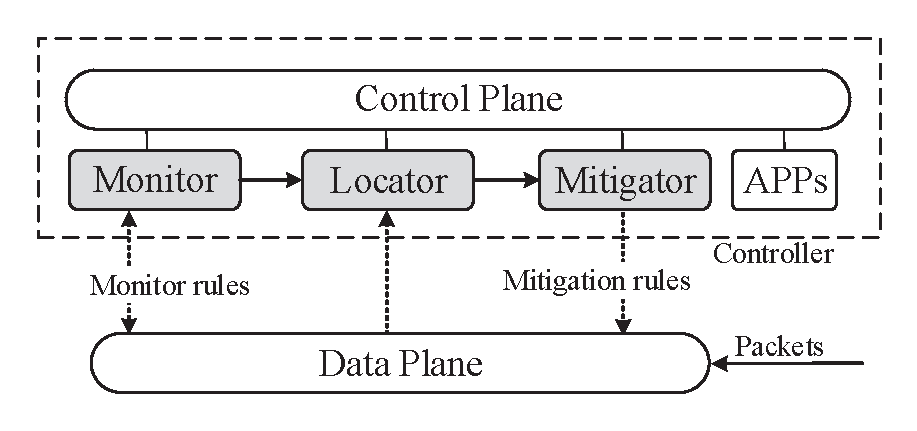
\includegraphics[scale=0.75]{architecture}
    \caption{基于带宽保障的LDoS防御方案流程图}
    \label{fig:architecture}
\end{figure}

\subsection{异常检测模块}
\label{chap4:Monitor}
异常检测模块的作用是在交换机上的每个端口处检测可能存在的LDoS攻击,并且激活其他模块来确认LDoS攻击。异常检测模块通过在每个交换机上安装检测流表规则在端口上来检测LDoS攻击。这些流表规则能够统计每个端口的TCP流的聚合吞吐量。异常检测模块通过周期性地获取这些流表规则的计数器数据就可以获知TCP流的聚合吞吐量变化情况。

异常检测模块首先从所有的数据包中分离出TCP数据包。然后,TCP数据包通过与这些特制的流表规则匹配,统计数据。接下来,再将这些TCP数据包转发给其他正常的流表规则进行处理。这些特制流表的匹配规则的匹配域加入转出端口信息,同时将优先级置为最高,以保证这些流表规则优先匹配数据包以统计TCP流的信息。接下来,特制的流表规则的指令为转发给其他正常流表规则进行处理,保证了这些流表规则只会统计TCP流的信息而不会干扰数据的传输。同时,异常检测模块需要把这些特制流表规则的idle\_timeout和hard\_timeout都设置为0以保证特制流表规则不会被删除,可以持续做数据的统计。

在交换机上安装特制流表规则后,异常检测模块按照算法\ref{alg:detection}检测TCP流的聚合吞吐量状态,若是TCP流的聚合吞吐量持续下降,则表示TCP流的聚合吞吐量下降明显,然后判断LDoS攻击是否可能出现,异常检测模块将会激活攻击定位模块来进行更深入精确的检测。算法\ref{alg:detection}展示了检测TCP吞吐量异常的伪代码。输入由吞吐量下降判定阈值$\alpha$和检测所得的序列$S$组成。输出为检测所得的结果$s$。$c$记录吞吐量持续下降的时间。如果$c$超过一个阈值$M$,$s$将会被标记为吞吐量异常,以此表示可能存在的LDoS攻击。同时检测到吞吐量异常的端口将被标记为异常端口。考虑控制器的带宽负载和模块的效率,设置异常检测模块的采样周期$T_s$为0.5秒,每次检测的时间长度为5秒。

\floatname{algorithm}{算法}
\renewcommand{\algorithmicrequire}{\textbf{输入:}}
\renewcommand{\algorithmicensure}{\textbf{输出:}}
\begin{algorithm}
	\small
	\caption{TCP流的聚合吞吐量异常检测}
	\label{alg:detection}
	\begin{algorithmic}[1]%ÿÐÐÏÔʾÐкÅ
	\Require $\alpha, S$;
	\Ensure $s$
	\State $c \gets 0$;
	\State $s \gets $吞吐量正常;
	\For{$(i=2 \rightarrow {len(S)})$}
		\If {$S_{i} < {\alpha} * S_{i - 1}$}
			\State $c \gets c + 1$;
		\Else 
			\State $c \gets 0$;
		\EndIf
		\If {$c {\ge} M$}
			\State $s \gets$ 吞吐量异常;
		\EndIf
	\EndFor
	\State \Return $s$
		
	\end{algorithmic}
\end{algorithm}

\subsection{攻击定位模块}
\label{chap4:Locator}

在异常检测模块激活了攻击检测模块之后,攻击检测模块对异常检测模块检测出的异常端口进行分析,确认LDoS攻击并识别LDoS攻击流。供给定位模块分为四个步骤。第一步,攻击定位模块对异常端口的总吞吐量进行二值化。第二步,攻击定位模块通过这些二值化后的吞吐量推断出异常端口吞吐量是否存在周期性。如果异常端口吞吐量存在周期性,则供给定位模块将确认异常端口正在被LDoS攻击所影响,因此,本文将确认被LDoS攻击所影响的端口称为受影响端口。攻击定位模块使用算法\ref{alg:port_locate}来确认异常端口是否为受影响端口。第三步,使用序列相似性来识别攻击流,通过平均欧式距离方法来判断攻击流。最后一步,找到攻击流的入口交换机上的端口,并且通知攻击限制模块来限制攻击流。




\subsubsection{吞吐量序列二值化}
\label{chap4:binarization}
通过采样获得的吞吐量序列在进行周期性判断之前需要进行处理。端口统计的数据包除了潜在的LDoS攻击数据包,也可能会包含在其他良性的流量影响周期性的判断。这些良性流量括三类:
\begin{itemize}
	\item 不会受到LDoS攻击和网络拥塞影响的UDP流
	\item LDoS未影响到的TCP流
	\item 其他经过该端口的更底层的数据流
\end{itemize}
这些良性流量不具备周期性,而且速率相较于LDoS的突发速率$R$要小很多。为了减少这些良性流量的影响,同时也为了更加便于提取周期性,攻击定位模块需要对流量进行二值化。攻击定位模块使用了阈值法进行二值化,假设该序列的最大吞吐量的值为$S_m$,设定二值化阈值为$\beta$,则吞吐量序列值中高于$\beta S_m$的地方置为1,吞吐量序列值中低于$\beta S_m$的地方置为0,这样就可以得到二值化序列。

\subsubsection{流量周期性检测}
为了确认LDoS攻击,攻击定位模块需要检测异常端口聚合流量周期$T$。所以,攻击定位模块能够通过检测二值化序列的周期$T_b$来推断周期$T$。假设某异常端口有周期为$T$的LDoS攻击流,控制器通过对异常端口的数据以合适的采样间隔$T_s$进行采样并进行二值化,获得二值化序列。通过提取二值化序列的功率谱密度的振幅最大值对应频率,就可以计算出二值化序列的周期$T_b$。LDoS攻击的$T$可以公式\ref{eqa:period}获得。

\begin{equation}
	\label{eqa:period}
	T = T_s * T_b
\end{equation}

如果采样间隔太大了,则公式计算出的LDoS攻击的$T$就会被放大而无法通过计算得出正确LDoS攻击流的$T$。根据奈奎斯特定理,只有在$T_s \le \frac{T}{2}$的条件下,攻击定位模块才能获得的正确的LDoS攻击流的$T$。因此,采样间隔需要足够小才能够满足需求。但是,随着采样间隔的减小,控制器需要收集处理的信息会增加,这样就会消耗很多控制信道的带宽和交换机的资源。因此,攻击定位模块在确认周期的时候只使用一个适合的固定采样间隔$T_s$。为了寻找合适的采样间隔,攻击定位模块将$T_s$初始化为$T_i$并且逐步减小$T_s$的取值直至计算出的$T$几乎不改变或者$T_s$比$T_e$更小。如果计算出的$T$几乎没有变化则能够确认LDoS攻击存在。如果$T_s$比$T_e$更小,则证明异常端口流量不存在LDoS攻击。在确认了LDoS攻击存在的情况下,将会在下一步中用$T_s$以确认攻击流而不是使用一个固定的值。这样,短周期的LDoS攻击也能够被检测。除此之外,检测长周期的LDoS攻击流引入的开销也会更加少。

如果一个异常端口被异常检测模块检测出来,攻击定位模块需要确认该端口是否受到LDoS攻击的影响。如果我们可以获得正确的LDoS攻击的$T$,则LDoS攻击就能够被确认。若是确认没有攻击,我们就终止攻击定位模块的流程,重新进入异常检测模块的流程。受影响的端口和攻击流都能够在功率谱密度的帮助下识别出来。为了尽量减少控制器的负担,攻击定位模块首先识别受影响端口,因为可能有很多流通过受影响端口,若是对每条流进行识别会消耗很多不必要的资源。最终,本文设计了一个适应性算法来识别受影响的端口。

\begin{algorithm}[H]
	\caption{动态搜索受影响的端口}
	\label{alg:port_locate}
	\begin{algorithmic}[1]
		\Require $~{\epsilon}, p$;
		\Ensure $s, T_s, T$;
		\State $T_s \gets T_i$;
		\State $T \gets \infty$; 
		\While{$T_s \ge T_e$}
		\State $seq \gets binarized\_sequence(T_s, p)$;
		\State $T_b \gets period\_extract(seq)$;
		\If {$abs(T - T_b * T_s)<\epsilon$}
		\State $s \gets$ 受影响;
		\State \Return $s, T_s, T$;
		\Else
		\State $T \gets T_b * T_s$;
		\State $T_s \gets T_s / 2$;
		\EndIf 
		\EndWhile
		\State $s \gets$ 不受影响;
		\State $T \gets 0$; 
		\State \Return $s, T_s, T$;
	\end{algorithmic}
\end{algorithm}

算法\ref{alg:port_locate}为识别受影响端口的伪代码。输入由可接受的计算周期误差$\epsilon$和一个异常端口$p$组成。输出由端口状态$s$,合适的采样周期$T_s$和推断出的LDoS攻击周期$T$。步骤1将$T_s$初始化为$T_i$。步骤2将$T$置为无穷大。主要的循环是步骤3至步骤13。在每一次的循环测试中一个$T_s$。步骤4以采样间隔$T_s$从异常端口$p$获得流量序列并二值化得到而二值序列$seq$。在步骤5中,通过分析功率谱提取二值序列$seq$的周期。步骤6至步骤8比较了两个不同采样频率下推断出的异常端口流量周期,如果两次推断出的周期的误差比可接受的计算周期误差$\epsilon$小,则可确定端口受LDoS攻击的影响。除此之外,还可以确定异常端口上有LDoS攻击流且攻击流的周期为$T$,此时的采样间隔为$T_s$。否则,按照步骤9至步骤11的进行处理,采样的频率变为原来的两倍,并将将要返回的$T$置为根据更低采样间隔的$T_s$推断出的$T$。步骤14至步骤16,将$T$置为0,并确定异常端口$p$未受LDoS攻击的影响。LDoS攻击的周期$T$可以通过合适的采样间隔$T_s$和公式\ref{eqa:period}获得。这样,算法\ref{alg:port_locate}通过不断降低的采样间隔计算端口流量的周期$T$直至获得$T$或者计算出端口流量没有周期性。

\subsubsection{二值化序列相似性}
\label{chap4:seq-similarity}

攻击定位模块在确定受影响的端口受到LDoS攻击的的影响后,开始对经过该端口的流进行分析,定位攻击者。在LDoS攻击的影响下,经过受影响端口的统计数据包大部分是LDoS攻击的数据包。因此,与其他正常数据流对比,LDoS攻击流的二值序列与受影响端口的二值化序列相似度是最高的。通过对经过受影响端口的所有流的二值化序列与该端口总流量的二值化序列的相似度进行比较,可以识别攻击流。获取二值化序列使用的采样间隔为算法\ref{alg:port_locate}所确认的$T_s$。假设异常端口的的二值化序列为$A$,一条经过该端口的数据流的二值化序列为$B$。假设$A$与$B$是同一时刻由交换机上传给控制器的,攻击定位模块将使用平均欧氏距离来衡量$A$与$B$的相似度。可以通过公式\ref{eq:euclidean_distance}获取平均欧氏距离。

\begin{equation}
	\vspace{-0.1in}
	\label{eq:euclidean_distance}
	\ MED=\frac{\sum_{i=1}^{N}\lvert A_{i} - B_{i}\rvert}{N}.
\end{equation}

LDoS攻击流的平均欧式距离小于正常流的平均欧式距离,因此,攻击定位模块能够使用一个二分类器来对流进行分类,供给定位模块使用阈值$\gamma$来区分流。平均欧氏距离小于$\gamma$的流将会被识别为攻击流。平局欧式距离大于$\gamma$的流将会被识别为正常流。在此处,不管LDoS攻击是由一个主机还是多个主机分布式完成的,都可以被检测,因此,攻击检测模块使用流级别的检测。


\subsubsection{攻击源入口定位}
\label{chap4:ingressportlocation}

攻击定位模块确定了LDoS攻击流之后,通过该流的流表规则所属的SDN中的路径可以锁定入口交换机和该流进入SDN网络的端口。然后攻击定位模块将LDoS攻击流的信息通知给攻击限制模块。攻击源可能是SDN网络中的主机,也可能是通过未知网络连接进入SDN网络的主机。对于不同的情况,攻击定位模块可以确认的信息是不同的。对于攻击源是SDN网络中的主机这种情况,攻击检测模块能够把攻击源直接连接的SDN交换机端口信息通知给攻击限制模块。对于第二种情况,攻击检测模块只能将连接未知网络的端口通知给攻击限制模块。

\subsection{攻击限制模块}
\label{chap4:Mitigator}

攻击限制模块的目的是限制LDoS攻击对SDN网络造成影响。因此,在识别LDoS攻击流之后,攻击限制模块将安装相应的限制规则对LDoS攻击进行处理。限制规则包括两种,一种为流表规则,一种是Meter规则。在攻击定位模块提供的LDoS攻击源信息的帮助下,攻击限制模块将在LDoS攻击的入口交换机处完成对于LDoS攻击的限制。攻击限制模块提供两种限制LDoS攻击的方法,阻塞攻击流和限制攻击流的速率。


\begin{figure}
    \centering
    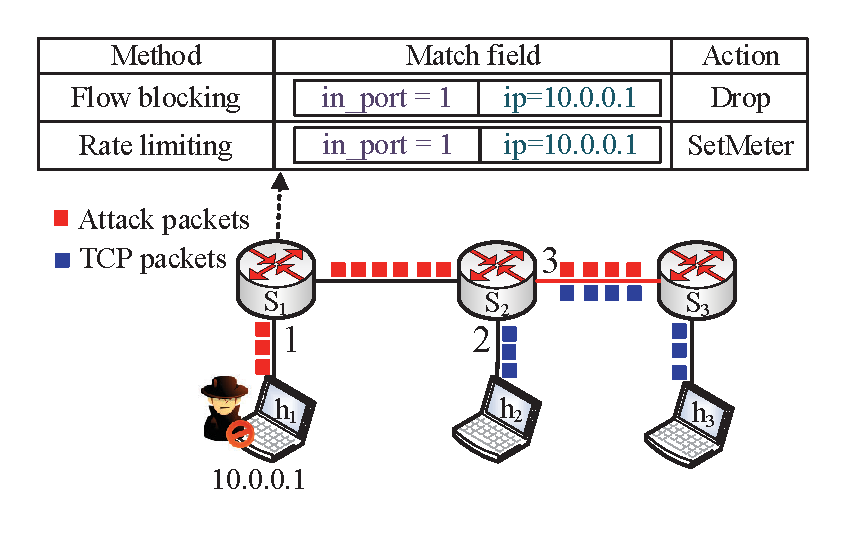
\includegraphics[scale=1]{defense}
    \caption{防御系统的一个例子,从$h_1$发送的LDos攻击流完全占用$S_2$与$S_3$之间连接的可用带宽。在$S_1$处,从$h_1$发送的LDoS攻击流被限制规则处理。}
    \label{fig:defense}
\end{figure}

图\ref{fig:defense}展示了攻击限制模块中限制规则的作用。在一个SDN网络中,攻击者$h_1$在交换机$S_1$的端口1处接入网络。合法用户$h_2$在在交换机$S_2$的端口2处接入网络。合法用户$h_3$在在交换机$S_3$的端口3处接入网络。假设$h_2$与$h_3$之间建立TCP连接,攻击者$h_1$想要完全占用$S_2$与$S_3$之间连接的可用带宽,并强迫$h_2$与$h_3$之间的TCP连接持续进入超时重传状态。在异常检测模块和攻击定位模块的帮助下,防御系统在$S_2$处识别了LDoS攻击,并且将攻击者$h_1$接入网络的端口1的信息通知给供给限制模块。攻击限制模块在入口交换机$S_1$处安装了相应的限制规则来阻塞或者限制$h_1$的流量。这样,攻击限制限制模块将完全消除LDoS攻击对于SDN网络的影响,$h_2$与$h_3$之间的TCP连接的吞吐量将会不在受到攻击者$h_1$的LDoS攻击的影响。

%Fig.~\ref{fig:mitigate} shows the mitigation method. The attacker $h_1$ accesses the network at port 1 and the legitimate user $h_2$ accesses the network at port 2 in the switch $S_1$. In addition, $h_2$ sends TCP packets to $h_3$. The attacker aims to overload the bandwidth of the link between $S_2$ and $S_3$ and thus to cause retransmission of the TCP flows between $h_2$ and $h_3$. The Locator module identifies the attack flow at $S_2$ and inform the Mitigator module on port 1. It blocks or limits the traffic of $h_1$ in the ingress switch $S_1$. Thus, the influence of the attack is eliminated and the TCP throughput of benign flows is not affected by the attack. 


由于LDoS攻击的特殊性,相应的限制规则是需要特别制定的。对于第一种方法,攻击限制模块想要阻塞LDoS攻击需要满足两个条件。首先安装在入口交换机的匹配LDoS攻击源的限制流表规则需要拥有最高的优先级,因为低优先级的限制规则会使一些攻击源的数据包避开限制流表规则而进入网络。因此,需要满足限制流表规则拥有所有流表规则中最高的优先级。其次,限制流表规则的指令必须是丢弃数据包,为了避免LDoS攻击的数据进入网络,最好的方案就是直接在交换机处丢弃攻击源的数据包。这样,在限制流表规则的作用下,LDoS攻击的数据包就无法进入网络,LDoS攻击将会被完全消除。但是,这也存在一定的风险,因为存在正常流量误判为攻击流的可能性,这些经过受影响端口的正常流也可能会受到影响。对于第二种方法,攻击限制模块使用了特制的Meter规则对LDoS攻击进行限制。对于限制LDoS攻击的Meter规则,burst\_size参数需要根据前面使用的$T_s$来特殊设置。攻击限制模块通过在入口交换机处安装特制的Meter规则,然后把与LDoS攻击流相关的流表规则与特制Meter规则绑定,就能达到限制LDoS突发速率的效果。

%For the first method, the flow rules that match the attack sources with the highest priority will be installed in the ingress switches. These rules block the attack flows at the ingress ports. The attack packets cannot be injected into the network anymore with the first method. Therefore, the influence of the attack will be eliminated. However, some benign traffic passing the blocked ingress ports may also be affected. In the second method, we leverage crafted meter rules, whose burst\_size is set based on $T_s$, for rate limitation. The Mitigator module assigns crafted meter rules to all the flow rules that match the attack traffic.

为了满足多种服务的需求,网络管理员根据不同的环境决定系统使用哪种方式限制LDoS攻击。一般情况下,阻塞LDoS攻击是限制LDoS攻击更好的方案。但是,管理者希望给所有主机保留一定的带宽以避免由于误判而对正常流的传输造成极大的影响。本系统默认的限制LDoS攻击的方法是阻塞LDoS流以保证SDN网络的安全性。

%To meet the various performance requirements, the network managers can determine which method is used in the system. In general, the first method is a better way to throttle the low-rate TCP attack. However, under the circumstances where the managers desire to reserve bandwidth for all the hosts, the second method is more suited to throttle the attack. The default method of our system is blocking the attack flows for the security of the network. 